
\documentclass[tikz,border=1pt]{standalone}

\usepackage{bm}

\usetikzlibrary{decorations.markings,arrows.meta}

%   電気力線のスタイル設定
\tikzset{eflineA/.style={thick,postaction=
    {decorate,decoration={
    markings, mark=at position 0.6 with {\arrow{Stealth}}}
    }}}
\tikzset{eflineB/.style={thick,postaction=
    {decorate,decoration={
    markings, mark=at position 0.616 with {\arrow{Stealth}}}
    }}}
\tikzset{eflineC/.style={thick,postaction=
    {decorate,decoration={
    markings, mark=at position 0.5 with {\arrow{Stealth}}}
    }}}
\tikzset{eflineD/.style={thick,postaction=
    {decorate,decoration={
    markings, mark=at position 0.653 with {\arrow{Stealth}}}
    }}}
\tikzset{eflineE/.style={thick,postaction=
    {decorate,decoration={
    markings, mark=at position 0.73 with {\arrow{Stealth}}}
    }}}
\tikzset{eflineF/.style={thick,postaction=
    {decorate,decoration={
        markings, mark=at position 0.81 with {\arrow{Stealth}},
        markings, mark=at position 0.22 with {\arrow{Stealth}}
    }}}}
\tikzset{eflineG/.style={thick,postaction=
    {decorate,decoration={
        markings, mark=at position 0.777 with {\arrow{Stealth}},
        markings, mark=at position 0.265 with {\arrow{Stealth}}
    }}}}
\tikzset{eflineH/.style={thick,postaction=
    {decorate,decoration={
        markings, mark=at position 0.76 with {\arrow{Stealth}},
        markings, mark=at position 0.29 with {\arrow{Stealth}}
    }}}}
\tikzset{eflineI/.style={thick,postaction=
    {decorate,decoration={
        markings, mark=at position 0.757 with {\arrow{Stealth}},
        markings, mark=at position 0.3 with {\arrow{Stealth}}
    }}}}

\tikzset{eflineA*/.style={thick,postaction=
    {decorate,decoration={
    markings, mark=at position 0.6 with {\arrow{Stealth[reversed]}}}
    }}}
\tikzset{eflineB*/.style={thick,postaction=
    {decorate,decoration={
    markings, mark=at position 0.616 with {\arrow{Stealth[reversed]}}}
    }}}
\tikzset{eflineC*/.style={thick,postaction=
    {decorate,decoration={
    markings, mark=at position 0.5 with {\arrow{Stealth[reversed]}}}
    }}}
\tikzset{eflineD*/.style={thick,postaction=
    {decorate,decoration={
    markings, mark=at position 0.653 with {\arrow{Stealth[reversed]}}}
    }}}
\tikzset{eflineE*/.style={thick,postaction=
    {decorate,decoration={
    markings, mark=at position 0.73 with {\arrow{Stealth[reversed]}}}
    }}}

\begin{document}

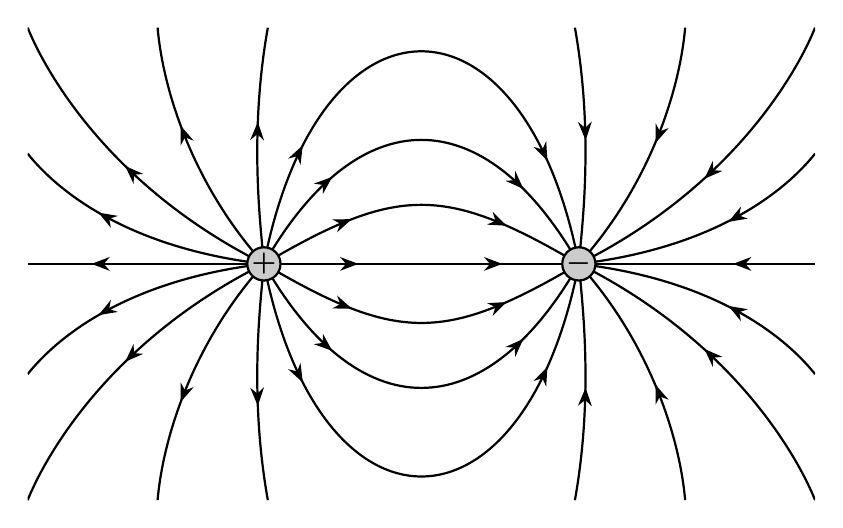
\begin{tikzpicture}

\pgfmathsetmacro{\xmax}{5}
\pgfmathsetmacro{\ymax}{3}

\pgfmathsetmacro{\X}{2}

\pgfmathsetmacro{\xa}{1.3}
\pgfmathsetmacro{\ya}{3.6}

\pgfmathsetmacro{\xb}{0.8}
\pgfmathsetmacro{\yb}{2.1}

\pgfmathsetmacro{\xc}{0.3}
\pgfmathsetmacro{\yc}{1}

\pgfmathsetmacro{\xd}{1.2}
\pgfmathsetmacro{\yd}{3}
\pgfmathsetmacro{\xe}{1.21}
\pgfmathsetmacro{\ye}{1.4}
\pgfmathsetmacro{\xf}{1.5}
\pgfmathsetmacro{\yf}{.8}

\pgfmathsetmacro{\xg}{1.95}
\pgfmathsetmacro{\yg}{3}
\pgfmathsetmacro{\xh}{2.2}
\pgfmathsetmacro{\yh}{1.6}
\pgfmathsetmacro{\xi}{2.03}
\pgfmathsetmacro{\yi}{0.4}

\pgfmathsetmacro{\xj}{3.35}
\pgfmathsetmacro{\yj}{3}
\pgfmathsetmacro{\xk}{3.28}
\pgfmathsetmacro{\yk}{2.2}
\pgfmathsetmacro{\xl}{2.9}
\pgfmathsetmacro{\yl}{1}

\pgfmathsetmacro{\xm}{5}
\pgfmathsetmacro{\ym}{3}
\pgfmathsetmacro{\xn}{4.8}
\pgfmathsetmacro{\yn}{2.5}
\pgfmathsetmacro{\xo}{4}
\pgfmathsetmacro{\yo}{1}

\pgfmathsetmacro{\xp}{5}
\pgfmathsetmacro{\yp}{1.4}
\pgfmathsetmacro{\xq}{4.6}
\pgfmathsetmacro{\yq}{0.9}
\pgfmathsetmacro{\xr}{3.7}
\pgfmathsetmacro{\yr}{0.2}

\begin{scope}\clip(-\xmax,-\ymax)rectangle(\xmax,\ymax);
    
    %   補助方眼
    %  \draw[step=1,thin,dotted] (-\xmax,-\ymax) grid (\xmax,\ymax);
    %  \draw[->] (-\xmax,0) -- (\xmax,0) node[right] {x};
    %  \draw[->] (0,-\ymax) -- (0,\ymax) node[above] {y};

    %   補助楕円
    %   \draw (-\X-0.5,0) circle [x radius=17mm, y radius=18.5mm];
    %   \draw (\X+0.5,0) circle [x radius=17mm, y radius=18.5mm];

    %   第2象限
    \draw[eflineA]
        (-\X,0)..controls(-\xi,\yi) and (-\xh,\yh)..(-\xg,\yg);
    \draw[eflineB]
        (-\X,0)..controls(-\xl,\yl) and (-\xk,\yk)..(-\xj,\yj);
    \draw[eflineC]
        (-\X,0)..controls(-\xo,\yo) and (-\xn,\yn)..(-\xm,\ym);
    \draw[eflineD]
        (-\X,0)..controls(-\xr,\yr) and (-\xq,\yq)..(-\xp,\yp);

    %   第3象限
    \draw[eflineA]
        (-\X,0)..controls(-\xi,-\yi) and (-\xh,-\yh)..(-\xg,-\yg);
    \draw[eflineB]
        (-\X,0)..controls(-\xl,-\yl) and (-\xk,-\yk)..(-\xj,-\yj);
    \draw[eflineC]
        (-\X,0)..controls(-\xo,-\yo) and (-\xn,-\yn)..(-\xm,-\ym);
    \draw[eflineD]
        (-\X,0)..controls(-\xr,-\yr) and (-\xq,-\yq)..(-\xp,-\yp);

    %   第1象限
    \draw[eflineA*]
        (\X,0)..controls(\xi,\yi) and (\xh,\yh)..(\xg,\yg);
    \draw[eflineB*]
        (\X,0)..controls(\xl,\yl) and (\xk,\yk)..(\xj,\yj);
    \draw[eflineC*]
        (\X,0)..controls(\xo,\yo) and (\xn,\yn)..(\xm,\ym);
    \draw[eflineD*]
        (\X,0)..controls(\xr,\yr) and (\xq,\yq)..(\xp,\yp);

    %   第4象限
    \draw[eflineA*]
        (\X,0)..controls(\xi,-\yi) and (\xh,-\yh)..(\xg,-\yg);
    \draw[eflineB*]
        (\X,0)..controls(\xl,-\yl) and (\xk,-\yk)..(\xj,-\yj);
    \draw[eflineC*]
        (\X,0)..controls(\xo,-\yo) and (\xn,-\yn)..(\xm,-\ym);
    \draw[eflineD*]
        (\X,0)..controls(\xr,-\yr) and (\xq,-\yq)..(\xp,-\yp);

    %   左右の水平な電気力線
    \draw[eflineE] (-\X,0) -- (-\xmax,0);
    \draw[eflineE*] (\X,0) -- (\xmax,0);

    
    %   中央の曲がった電気力線
    \draw[eflineF]
        (-\X,0)..controls(-\xa,\ya) and (\xa,\ya)..(\X,0);
    \draw[eflineG]
        (-\X,0)..controls(-\xb,\yb) and (\xb,\yb)..(\X,0);
    \draw[eflineH]
        (-\X,0)..controls(-\xc,\yc) and (\xc,\yc)..(\X,0);
    \draw[eflineF]
        (-\X,0)..controls(-\xa,-\ya) and (\xa,-\ya)..(\X,0);
    \draw[eflineG]
        (-\X,0)..controls(-\xb,-\yb) and (\xb,-\yb)..(\X,0);
    \draw[eflineH]
        (-\X,0)..controls(-\xc,-\yc) and (\xc,-\yc)..(\X,0);
    
    %   中央の水平な電気力線
    \draw[eflineI] (-\X,0) -- (\X,0);

    %   左の点電荷（＋）
    \draw[thick,fill=gray!40] (-\X,0) circle(6pt); 
    \node at (-\X,0) {$\bm{+}$};

    %   右の点電荷（－）
    \draw[thick,fill=gray!40] (\X,0) circle(6pt); 
    \node at (\X,0) {$\bm{-}$};

\end{scope}

\end{tikzpicture}

\end{document}

